%%%%%%%%%%%%%%%%%%%%%%%%%%%%%%%%%%%%%%%%%%
% Engineering problems / LaTeX Template
%		Semester 6
%		Institut d'Optique Graduate School
%%%%%%%%%%%%%%%%%%%%%%%%%%%%%%%%%%%%%%%%%%
%	6N-IntNum-BlocRobot	/ Embedded System
%%%%%%%%%%%%%%%%%%%%%%%%%%%%%%%%%%%%%%%%%%
%
% Created by:
%	Julien VILLEMEJANE - 05/nov/2026	
%
%%%%%%%%%%%%%%%%%%%%%%%%%%%%%%%%%%%%%%%%%%
% Professional Newsletter Template
% LaTeX Template
% Version 1.0 (09/03/14)
%
% Created by:
% Bob Kerstetter (https://www.tug.org/texshowcase/) and extensively modified by:
% Vel (vel@latextemplates.com)
% 
% This template has been downloaded from:
% http://www.LaTeXTemplates.com
%
% License:
% CC BY-NC-SA 3.0 (http://creativecommons.org/licenses/by-nc-sa/3.0/)
%
%%%%%%%%%%%%%%%%%%%%%%%%%%%%%%%%%%%%%%%%%

\documentclass[a4paper,11pt,titlepage]{article} % The default font size is 10pt; 11pt and 12pt are alternatives

%%%%%%%%%%%%%%%%%%%%%%%%%%%%%%%%%%%%%%%%%%%%%%%%%%%%%%%%%%%%%%%%%%%%%%%%%%%%%%%%%%%%%%%%%%%%%%%%%%%%%%%%%%%%%%%%%%%%%%%%%%%%%%%%%%%%%%%%%%%%%%%%%%%%%%%%%%%%%%%%%%%%%%%%%%%%%%%%%%%%%%%%%%%%%%%%%%%%%%%%%%%%%%%%%%%%%%%%%%%%%%%%%%%%%%%%%%%%%%%%%%%%%%%%%%%%
\usepackage{opto_elec_villemejane}
\usetikzlibrary{positioning}

%%%%%%%%%%%%%%%%%%%%%%%%%%%%%%%%%%%%%%%%%%%%%%%%
%%%%%%%%%%%%%%%%%%%%%%%%%%%%%%%%%%%%%%%%%%%%%%%%
\begin{document}



% Page de garde
\begin{titlepage}

\begin{center}
	\begin{minipage}{2.5cm}
	\begin{center}
		
\includegraphics[width=8cm]{images/Logo-LEnsE.png}
	\end{center}
\end{minipage}\hfill
\begin{minipage}{10cm}
	\begin{center}
	\textbf{Institut d'Optique Graduate School }\\[0.1cm]
    \textbf{\textsc{\Large Interfaçage Numérique}}


	\end{center}
\end{minipage}\hfill


\vspace{1cm}

{\large \bfseries Travaux Pratiques} \\[0.2cm]
Semestre 6

\vspace{2cm}
% Title
\rule{\linewidth}{0.3mm} \\[0.4cm]
{ \huge \bfseries\color{violet_iogs} Banc de mesure de rayonnement \\[0.4cm] }
\rule{\linewidth}{0.3mm} \\[1cm]

2 séances

\bigskip

\begin{center}
	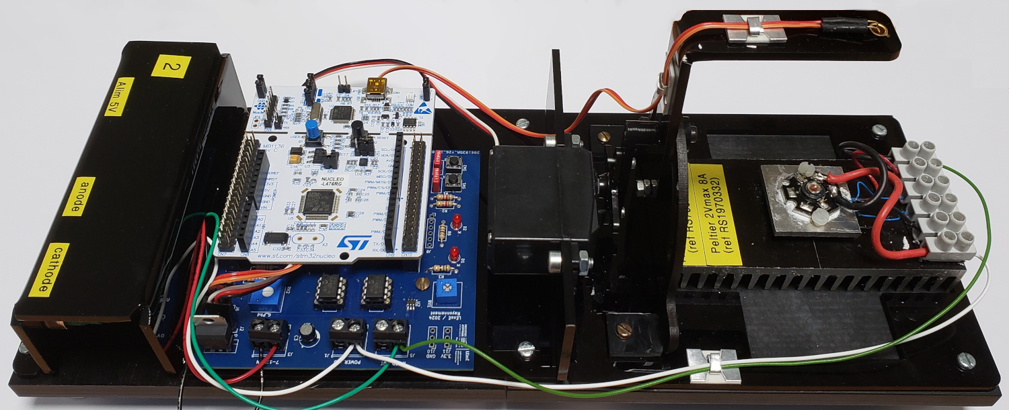
\includegraphics[width=0.7\textwidth]{images/rayonnement.png}
\end{center}

\vfill

\textit{Ce sujet est disponible au format électronique sur le site du LEnsE - https://lense.institutoptique.fr/ dans la rubrique Année / Première Année / Interfaçage Numérique S6 / Bloc 3 – Interface d'acquisition de données.}

\vspace{1.5cm}

\begin{minipage}{5cm}
\begin{center}

\includegraphics[width=3cm]{./images/logocc}\\
\small
  © 2026 by LEnsE-IOGS 
\end{center}
\end{minipage}
% Bottom of the page
%{\textbf{\large {Année universitaire} 2024-2025}}

\end{center}
\end{titlepage}

\newpage
\strut % empty page


%%%%%%%%%%%%%%%%%%%%%%%%%%%%%%%%%%%%%%%%%%%%%%%%
%%%%%%%%%%%%%    Intro
\newpage
\pagestyle{empty}

\begin{minipage}[c]{.25\linewidth}
	
\includegraphics[width=5cm]{images/Logo-LEnsE.png}
\end{minipage} \hfill
\begin{minipage}[c]{.4\linewidth}

\begin{center}
\vspace{0.3cm}
{\Large \textsc{Interfaçage Numérique}}

\medskip

6N-047-SCI \qquad \textbf{\large Bloc Rayonnement}

\end{center}
\end{minipage}\hfill

\vspace{0.5cm}

\noindent \rule{\linewidth}{1pt}

{\noindent\Large  \rule[-7pt]{0pt}{30pt} \textbf{Banc de mesure de rayonnement}}

\noindent \rule{\linewidth}{1pt}

\bigskip 

%%%%%%%%%%%%%%%%%%%%%%%%%%%%%%%%%%%%%%%%%%%%%%%%
%%%%%%%%%%%%%    A A V

{\large À l'issue des séances de TP concernant le \textbf{bloc d'acquisition d'un diagramme de rayonnement}, les étudiant$\cdot$es seront capables de :}

\medskip

\begin{itemize}	
	\item Développer, mettre en \oe{}uvre et valider une \textbf{solution informatique pour acquérir des données} selon un protocole établi
	\item Mettre en \oe{}uvre un \textbf{protocole simple de communication} entre un ordinateur et un microcontrôleur pour transmettre des commandes et lire des données
	\item Documenter un programme informatique
	\item Etablir un \textbf{protocole de test}, réaliser les tests et rédiger une \textbf{analyse préliminaire des résultats}
\end{itemize}

\noindent \rule{\linewidth}{1pt}


%%%%%%%%%%%%%%%%%%%%%%%%%%%%%%%%%%%%%%%%%%%%%%%%
%%%%%%%%%%%%%    Objectifs

\section{Objectifs du mini-projet}

L'objectif principal de ce mini-projet est d'\textbf{automatiser un banc de mesure de rayonnement lumineux} à l'aide d'un ordinateur et d'une interface en Python. Le matériel est piloté par une carte à microcontroleur à laquelle il faudra envoyer des commandes selon un protocole série donné.

\medskip

Un diagramme de rayonnement lumineux est la \textbf{représentation graphique} de la \textbf{distribution angulaire} d'une grandeur caractérisant le rayonnement d'une source lumineuse.

\begin{center}
	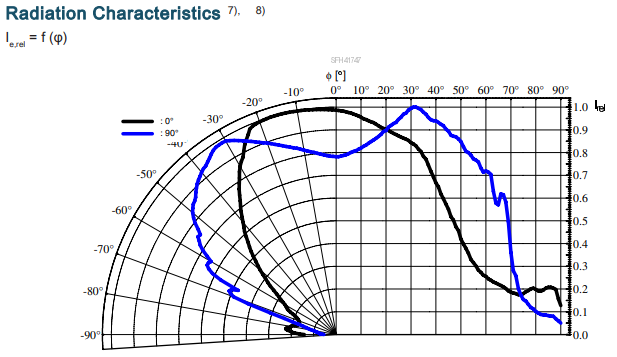
\includegraphics[width=0.7\textwidth]{images/osram_sfh41747.png}
	
	Exemple de diagramme de rayonnement d'une LED OSRAM SFH 41747 (documentation technique)
\end{center}


\medskip

Vous aurez à votre disposition une \textbf{maquette} permettant la mise en mouvement d'un système de photodétection autour d'une source de puissance à LED. Cette maquette est pilotée par une carte Nucléo (contenant un microcontroleur).


%%%%%%%%%%%%%%%%%%%%%%%%%%%%%%%%%%%%%%%%%%%%%%%%
%%%%%%%%%%%%%    Déroulement

\section{Déroulement du bloc}

\subsection{Séance 1 / Prise en main de la maquette et du protocole}

	\begin{description}
		\item[Etape A] Etude de la maquette et du protocole
		\item[Etape B] Liaison série et python
	\end{description}

\subsection{Séance 2 / Mise en place de l'application d'acquisition}

	\begin{description}
		\item[Etape C] Application d'acquisition en Python
		\item[Etape D] Essai sur une LED de puissance
	\end{description}

\medskip

\textit{Selon le temps restant, il sera possible d'intégrer les fonctions écrites en Python dans une interface graphique, dont la structure de base est fournie.}

%%%%%%%%%%%%%%%%%%%%%%%%%%%%%%%%%%%%%%%%%%%%%%%%
%%%%%%%%%%%%%    DISC

\section{DISC / Accumulation de preuves}

Nous vous rappelons également que l'un des livrables final de ce module est un \textbf{Document Individuel de Suivi de Compétences} qui devra revendiquer votre progression dans l'acquisition des compétences suivantes :

\begin{itemize}
	\item C4 – Valider une solution technologique
	\item C7 – Travailler en équipe
\end{itemize}

\subsection{Travail à réaliser}

Vous devrez donc tout au long des séances de TP : 

\begin{itemize}
	\item Documenter les tests réalisés pour valider les fonctionnalités mise en oeuvre
	\item Stocker les preuves pour revendiquer la montée en compétences (résultats, photos, vidéos...)
\end{itemize}



%%%%%%%%%%%%%%%%%%%%%%%%%%%%%%%%%%%%%%%%%%%%%%%%
%%%%%%%%%%%%%    DISC

\section{Ressources}


Des fichiers binaires, des codes en C++ et des scripts en Python sont à télécharger tout au long des séances de TP. Vous les trouverez sur le site du LEnsE :

\textbf{Année / Première Année / Interfaçage Numérique S6 / Bloc 3 – Interface d'acquisition de données / Exemples de codes}


\cleardoublepage
\strut % empty page
%%%%%%%%%%%%%%%%%%%%%%%%%%%%%%%%%%%%%%%%%%%%%%%%
%%%%%%%%%%%%%    Séance 2 détaillée

\begin{minipage}[c]{.25\linewidth}
	
\includegraphics[width=4cm]{images/Logo-LEnsE.png}
\end{minipage} \hfill
\begin{minipage}[c]{.4\linewidth}

\begin{center}
\vspace{0.3cm}
{\Large \textsc{Interfaçage Numérique}}

\medskip

6N-047-SCI \qquad \textbf{\large Bloc Rayonnement}

\end{center}
\end{minipage}\hfill

\vspace{0.5cm}

\noindent \rule{\linewidth}{1pt}

{\noindent\Large \rule[-7pt]{0pt}{30pt} Séance 1 / Prise en main de la maquette et du protocole} 

\noindent \rule{\linewidth}{1pt}


%%%%%%%%%%%%%%%%%%%%%%%%%%%%%%%%%%%%%%%%%%%%%%%%
%%%%%%%%%%%%%    Maquette
\section{Description de la maquette}

La maquette est constituée :

\begin{itemize}
	\item d'une source de lumière, une LED de puissance
	\item d'une photodiode BPX65, associée à un circuit de photodétection simple
	\item d'un servomoteur, permettant de positionner le bras supportant la photodiode au dessus de la source lumineuse selon un angle donné (de -90° à +90°, par pas minimal de 1°)
	\item d'une carte de contrôle associée à une carte Nucléo L476RG
\end{itemize}

\begin{center}
	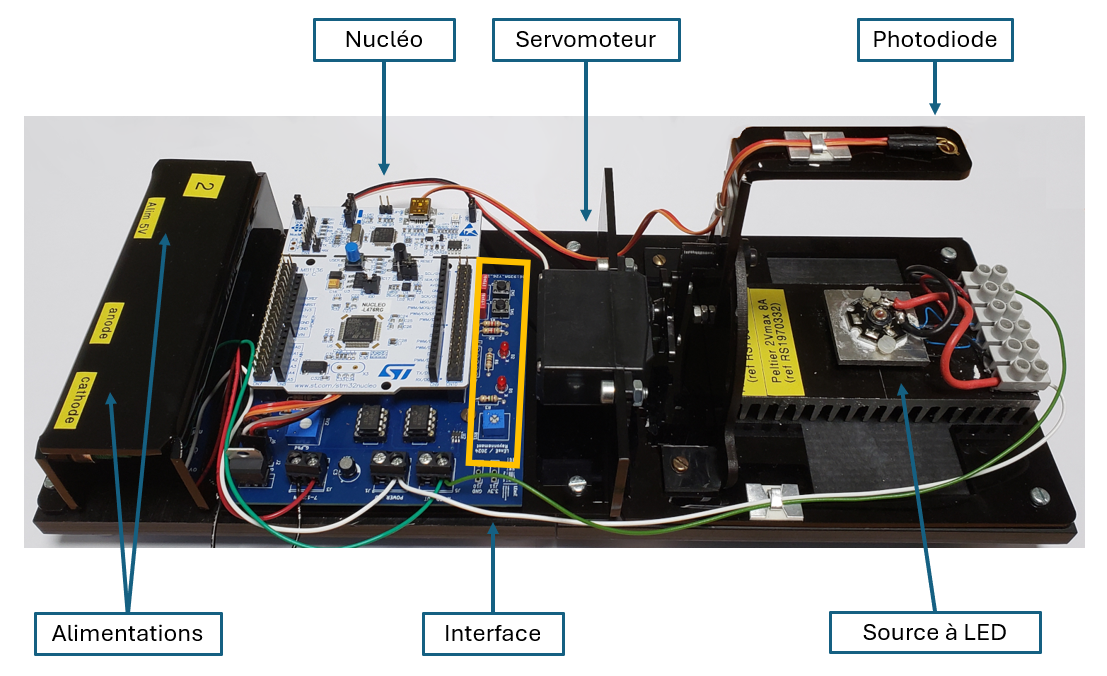
\includegraphics[width=0.8\textwidth]{images/maquette_rayon.png}
\end{center}


\subsection{Alimentation électrique}

Les bornes d'alimentation notées \textbf{Alim} $7\operatorname{V}$ permet d'alimenter le servomoteur.

Les bornes notées \textbf{anode} et \textbf{cathode} permettent d'alimenter la LED de puissance.

\medskip

\noindent \rule{\linewidth}{1pt}

{\LARGE La tension maximale admissible par le servomoteur est de $7\operatorname{V}$ !}

La tension minimale est de $5.5\operatorname{V}$

\medskip

{\Large Le courant maximal admissible par la LED de puissance est de $200\operatorname{mA}$ !}

\noindent \rule{\linewidth}{1pt}



\newpage


%%%%%%%%%%%%%%%%%%%%%%%%%%%%%%%%%%%%%%%%%%%%%%%%
%%%%%%%%%%%%%    Objectifs
\section{Protocole de communication}

Un \textbf{protocole de communication} est un ensemble de règles, de conventions et de formats définis pour permettre l'échange d'informations entre différents systèmes. Il détermine comment les données sont structurées, envoyées, reçues et interprétées par les parties communicantes.

Dans le cas de cette application, l'ordinateur, maitre de la communication, devra envoyer des commandes à la carte embarquée, qui devra les exécuter puis acquitter du bon déroulement de l'opération.


% Diagramme
\begin{center}
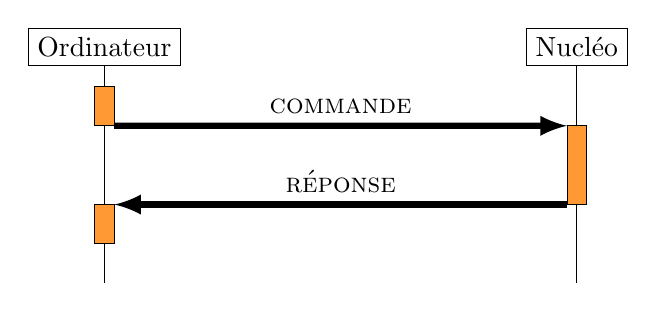
\begin{tikzpicture}

%% Locations
\def\PCToMCU{++(6,0)}
\def\MCUToPC{++(-6,0)}
\def\Lifeline{++(0,-3)}

%% Lifelines
\path (0,0)           node[draw] (PC) {Ordinateur}
      \PCToMCU node[draw] (MCU) {Nucléo};
\draw (PC) -- \Lifeline (MCU) -- \Lifeline;

%% Blocks
\path (PC)
      ++(0,-0.5) node (BeginProcess1) {} node[below right] {}
      ++(0,-0.5) node (EndProcess1)   {};
\filldraw[fill=orange!80] (BeginProcess1.east) rectangle (EndProcess1.west);

\path (MCU)
      ++(0,-1) node (BeginProcess2) {} node[below right] {}
      ++(0,-1) node (EndProcess2)   {};
\filldraw[fill=orange!80] (BeginProcess2.west) rectangle (EndProcess2.east);

\path (PC)
      ++(0,-2) node (BeginProcess3) {} node[below right] {}
      ++(0,-0.5) node (EndProcess3)   {};
\filldraw[fill=orange!80] (BeginProcess3.east) rectangle (EndProcess3.west);

%% Calls
\draw[->, line width=0.8mm, >=latex] (EndProcess1.east) -- node[above] {\textsc{commande}} (BeginProcess2.west);
\draw[->, line width=0.8mm, >=latex] (EndProcess2.west) -- node[above] {\textsc{réponse}} (BeginProcess3.east);

\end{tikzpicture}
\end{center}

\medskip

Il est important lorsqu'on souhaite \textbf{construire un protocole de communication} de :

\begin{itemize}
	\item \textbf{choisir un protocole de bas niveau} pour la transmission des commandes et des réponses
	\item définir la \textbf{structure des commandes}
	\item planifier la \textbf{liste des commandes}
	\item coder la récupération des données sur la carte Nucléo (et tester avec un moniteur Série)
	\item coder l'envoi des commandes sur le PC (en Python par exemple)
\end{itemize}


\subsection{Choix du protocole de bas niveau}

Nous utiliserons dans le cas de notre application la \textbf{liaison Série} (ou RS232).

Le protocole RS-232 est une \textbf{norme de communication série asynchrone} point à point qui permet de relier un équipement terminal de traitement de données (comme un ordinateur) à un équipement de terminaison de circuit de données (comme un instrument de mesure).

\begin{center}
	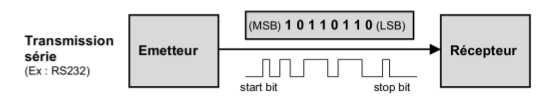
\includegraphics[width=0.7\textwidth]{./images/serial_link.png}
\end{center}

Il permet la communication entre deux noeuds d'un réseau, selon une trame structurée de la façon suivante : 1 bit de \textit{start}, 8 bits de données (en règle générale), 1 bit de parité optionnel (pair ou impair), 1 à 2 bits de stop.

\begin{center}
	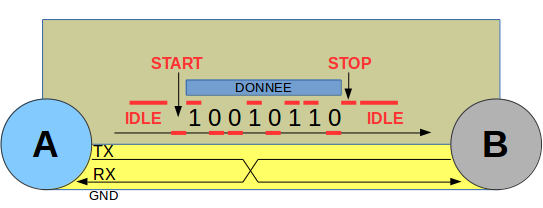
\includegraphics[width=0.5\textwidth]{./images/serial_rs_232.png}
\end{center}

\bigskip

\textit{Nous utiliserons le logiciel \textbf{Tera Term} afin de pouvoir visualiser et transmettre des données au format RS-232 à la maquette.}


\newpage
%%%%%%%%%%%%%%%%%%%%%%%%%%%%%%%%%%%%%%%%%%%%%%%%
%%%%%%%%%%%%%    Etape A
\section{Etape A / Etude de la maquette et du protocole}

\Manip Connecter la maquette à l'aide du câble USB.

\medskip

\textit{Elle est par la suite reconnue comme un périphérique de stockage USB, dans lequel vous pourrez \textbf{déplacer les fichiers binaires} à télécharger tout au long des différentes étapes.}

\subsection{A.1 / Etude du protocole de bas niveau}

Le protocole choisi est RS-232 (voir page précédente). Il permet d'envoyer un caractère ASCII à la fois.

\medskip

L'exemple, que nous allons étudier dans un premier temps, se base sur un protocole simplifié, ne nécessitant l'envoi que d'\textbf{un seul caractère par commande}.

\Manip Télécharger le fichier \textsl{test\_comm\_led.bin} (dans les ressources du TP sur le site du LEnsE). Copier-le dans sur la carte Nucléo de la maquette.

\medskip

\Manip Lancer le logiciel \textbf{Tera Term}. Sélectionner, dans la partie \textbf{Série}, le port de communication correspondant à la carte Nucléo (STM32...).

\Manip Sur le logiciel \textbf{Tera Term} :

\begin{itemize}
	\item cocher l'option \textsl{Echo Local} dans le menu \textsl{Configuration / Terminal}
	\item modifier la vitesse de transfert à \textbf{115200 bauds} dans le menu \textsl{Configuration / Port Série...} 
\end{itemize}

\Manip Dans \textbf{Tera Term}, envoyer les caractères 'a', 'e' et 'z' à la maquette. Observer ce qui se passe sur les différentes LEDs (D1 et D2).

\medskip

\Manip Changer la vitesse de transfert à 9600 bauds et tester à nouveau l'envoi des commandes. Que se passe-t-il ?

\medskip

Le code embarqué dans la maquette est fourni dans le fichier \textsl{test\_comm\_led.cpp} (dans les ressources du TP sur le site du LEnsE). 

\Manip Télécharger ce fichier et l'ouvrir avec un éditeur de texte.

\Quest Faire un schéma de principe du fonctionnement de ce code et des échanges entre le PC et la maquette.


\subsection{A.2 / Protocole complet}

Le protocole de bas niveau ne suffit pas lorsqu'on souhaite envoyer des commandes (ou des données) plus complexes qu'un simple caractère.

Il est alors essentiel de mettre en place un \textbf{protocole de plus haut niveau}.

\medskip

\textit{La \textbf{liste des commandes} utiles pour la maquette sont disponibles en annexe de ce document.}

\subsubsection{Structure des commandes}

Chaque commande doit avoir un \textbf{format bien défini} pour que l'instrument piloté puisse la comprendre et la traiter.

\begin{center}
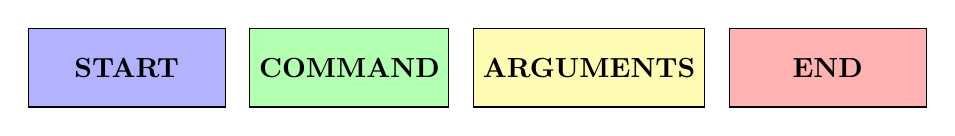
\begin{tikzpicture}[font=\sffamily]

%% Styles des blocs
\tikzstyle{block} = [rectangle, draw, minimum width=2.5cm, minimum height=1.0cm, align=center, font=\bfseries]

%% Blocs
\node[block, fill=blue!30] (start) {START};
\node[block, fill=green!30, right=0.3cm of start] (command) {COMMAND};
\node[block, fill=yellow!30, right=0.3cm of command] (arguments) {ARGUMENTS};
\node[block, fill=red!30, right=0.3cm of arguments] (end) {END};

\end{tikzpicture}
\end{center}

La liaison Série étant asynchrone, il est indispensable de prévoir dans le protocole des \textbf{caractères de début et de fin} de chaines de commande et de réponse.

\subsubsection{Commande}

Par exemple, on pourra se baser sur la structure suivante pour le cas d'une commande (entre le PC et le microcontroleur) :

\begin{center}
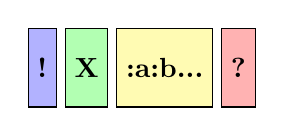
\begin{tikzpicture}[font=\sffamily]

%% Styles des blocs
\tikzstyle{block} = [rectangle, draw, minimum height=1.0cm, align=center, font=\bfseries]

%% Blocs
\node[block, fill=blue!30] (start) {!};
\node[block, fill=green!30, right=0.1cm of start] (command) {X};
\node[block, fill=yellow!30, right=0.1cm of command] (arguments) {:a:b...};
\node[block, fill=red!30, right=0.1cm of arguments] (end) {?};

\end{tikzpicture}
\end{center}

\textit{Les arguments sont facultatifs, selon les commandes.}

\subsubsection{Réponse}

Par exemple, on pourra se baser sur la structure suivante pour le cas d'une réponse (entre le PC et le microcontroleur) :

\begin{center}
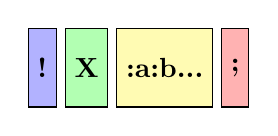
\begin{tikzpicture}[font=\sffamily]

%% Styles des blocs
\tikzstyle{block} = [rectangle, draw, minimum height=1.0cm, align=center, font=\bfseries]

%% Blocs
\node[block, fill=blue!30] (start) {!};
\node[block, fill=green!30, right=0.1cm of start] (command) {X};
\node[block, fill=yellow!30, right=0.1cm of command] (arguments) {:a:b...};
\node[block, fill=red!30, right=0.1cm of arguments] (end) {;};

\end{tikzpicture}
\end{center}

\textit{Les arguments sont facultatifs, selon les commandes.}


\subsubsection{Réponse}


%%%%%%%%%%%%%%%%%%%%%%%%%%%%%%%%%%%%%%%%%%%%%%%%
%%%%%%%%%%%%%    Etape B
\section{Etape B / Liaison série et python}


\subsection{B.1 / Premiers échanges - protocole de bas niveau}


On propose de remplacer la console Série par un \textbf{script Python} contenu dans le fichier \textsl{test\_comm\_led.py}.

\Manip Exécuter ce script python.

\subsection{Transmission des données par liaison série}


\cleardoublepage
\strut % empty page
%%%%%%%%%%%%%%%%%%%%%%%%%%%%%%%%%%%%%%%%%%%%%%%%
%%%%%%%%%%%%%    Séance 3 détaillée

\begin{minipage}[c]{.25\linewidth}
	
\includegraphics[width=4cm]{images/Logo-LEnsE.png}
\end{minipage} \hfill
\begin{minipage}[c]{.4\linewidth}

\begin{center}
\vspace{0.3cm}
{\Large \textsc{Interfaçage Numérique}}

\medskip

6N-047-SCI \qquad \textbf{\large Bloc Rayonnement}

\end{center}
\end{minipage}\hfill

\vspace{0.5cm}

\noindent \rule{\linewidth}{1pt}

{\noindent\Large \rule[-7pt]{0pt}{30pt} Séance 3 / Mise en place d'un protocole de communication} 

\noindent \rule{\linewidth}{1pt}





\subsection{Pilotage de la LED de puissance}

\Manip Alimenter la LED de puissance avec un courant maximal de 200mA. 

\bigskip

\textbf{\textit{Attention ! Paramètrer l'alimentation de la LED pour ne pas dépasser 200mA !}}

\textbf{\textit{Attention également à vos yeux...}}

\textit{Et brancher la LED dans le bon sens... Cathode = point de plus faible potentiel.}

\subsection{Premier diagramme de rayonnement}

\Manip Faire l'acquisition des valeurs d'intensité lumineuse pour des angles allant de $0$ à $180^\circ{}$ par pas de $10^\circ{}$ et transmettre les données par liaison Série à l'ordinateur.





%%%%%%%%%%%%%%%%%%%%%%%%%%%%%%%%%%%%%%%%%%%%%%%%
%%%%%%%%%%%%%    Etape 10
\section{Etape 11 / Mettre en place un protocole de communication basé sur une liste de commandes}

\subsection{Envoi et réception de messages simples}

Avant de se lancer dans la mise en place du protocole complet, nous vous proposons de tester l'exemple donné dans le fichier \textsl{test\_comm\_led.cpp}. Cet exemple se base sur un protocole simplifié, ne nécessitant l'envoi que d'\textbf{un seul caractère par commande}.

\Manip Tester le code fourni en envoyant des lettres par l'intermédiaire d'une console Série (logiciel \textbf{TeraTerm} par exemple).

\Quest A quel moment est appelée la fonction \textsl{ISR\_my\_pc\_reception()} ? A quoi sert-elle ?

\bigskip

On propose de remplacer la console Série par un \textbf{script Python} contenu dans le fichier \textsl{test\_comm\_led.py}.

\Manip Exécuter ce script python.


\subsection{Structure de base}

On se propose de tester le code \textsl{test\_version\_a\_d.cpp}. Ce fichier est disponible sur le site du LEnsE dans la rubrique \textit{Année / Première Année / Interfaçage Numérique S6 / Banc de mesure de rayonnement lumineux / Exemples de Codes}.

\Manip Compiler ce code et le téléverser sur la carte Nucléo.

\Quest A quoi sert la fonction \textsl{is\_angle\_ok()} ?

\Manip Ouvrir le logiciel TeraTerm et envoyer la commande suivante : \textsc{!A:10?}.

\Quest Que renvoie la carte Nucléo ? Expliquer les fonctions \textsl{ISR\_my\_pc\_reception()} (vis-à-vis du choix de la structure d'une commande) et la boucle infinie. On s'intéressera notamment aux changements de valeur des variables \textsl{string\_complete} et \textsl{input\_cnt}.

\Quest Que se passe-t-il lorsqu'on transmet une mauvaise valeur (soit avec la commande A, soit avec la commande D) ?

\Quest Faire un algorigramme du code.

\subsection{Ajout des autres commandes}

On souhaite à présent compléter ce code pour pouvoir traiter l'ensemble des commandes mentionnées dans la section précédente (T, A, B, C, S, E, D).

\Manip Compléter le code précédent et le tester.

\Quest A quel moment doit-on utiliser la \textbf{fonction d'acquisition} réalisée à l'étape 8 ? D'autres commandes sont-elles acceptables lors de l'acquisition ? Comment bloquer l'exécution des autres commandes ?

\Manip Mettre en place ce blocage.

\Quest A quel moment doit-on utiliser la \textbf{fonction de transmission} des données réalisée à l'étape 9 ?

\newpage
\subsection{Test complet}

\Quest Quelle est la suite de commandes à transmettre à la carte Nucléo pour permettre l'acquisition de données pour des angles allant de $-40^\circ{}$ à $+60^\circ{}$ par pas de $10^\circ{}$ et la récupération des données sur le moniteur Série ?

\Quest Tracer le diagramme de séquence associé à ces échanges de commandes et de réponses entre le PC et la carte Nucléo.

\Manip Tester l'acquisition de cette série de données.


%%%%%%%%%%%%%%%%%%%%%%%%%%%%%%%%%%%%%%%%%%%%%%%%
%%%%%%%%%%%%%    Etape 11
\section{Etape 12 / Utiliser la bibliothèque pySerial en Python pour envoyer les commandes à la carte Nucléo}


\begin{mdframed}[style=sidebar,frametitle={}]
\large
\textbf{ATTENTION} / Lors de l'utilisation d'un script Python nécessitant l'accès à la liaison Série, le logiciel \textbf{TeraTerm} doit être \textbf{fermé}.
\end{mdframed}


\medskip

On se propose à présent d'utiliser un script en langage Python pour pouvoir transmettre les commandes et recevoir les données sur l'ordinateur. Nous utiliserons la bibliothèques \textbf{pySerial} (à installer par la commande \textsl{pip install pyserial} dans une console ou un prompt d'Anaconda).

\medskip

Un code de base, nommé \textsl{test\_version\_a\_d.py}, est disponible sur le site du LEnsE dans la rubrique \textit{Année / Première Année / Interfaçage Numérique S6 / Banc de mesure de rayonnement lumineux / Exemples de Codes}.

\medskip

\Manip Exécuter ce code et tester les deux commandes pré-configurées ('a' et 'd').

\Manip A partir de cet exemple, réaliser un script qui permette de lancer l'acquisition de données pour des angles allant de $-40^\circ{}$ à $+60^\circ{}$ par pas de $10^\circ{}$ et la récupération des données acquises dans une liste en Python.

\Manip Afficher les données obtenues sur un graphique à l'aide de Matplotlib. Générer l'axe des angles.


%%%%%%%%%%%%%%%%%%%%%%%%%%%%%%%%%%%%%%%%%%%%%%%%
%%%%%%%%%%%%%    Etape 12
\section{Etape 13 / Tester la communication entre la carte Nucléo et le script Python pour afficher les données}

On souhaite enfin créer une application en console complète permettant à l'utilisateur de saisir les angles de départ et de fin, le pas angulaire et de lancer l'acquisition. Votre application devra ensuite afficher les données acquises.

Vous pourrez faire plusieurs essais avec des courants dans la LED de puissance de $50\operatorname{mA}$, $100\operatorname{mA}$ et $200\operatorname{mA}$ par exemple.


\newpage
%%%%%%%%%%%%%%%%%%%%%%%%%%%%%%%%%%%%%%%%%%%%%%%%
%%% RESSOURCES COMPLEMENTAIRES		

\newpage
% Ressources
\begin{center}
	\begin{minipage}{2.5cm}
	\begin{center}
		
\includegraphics[width=5cm]{images/Logo-LEnsE.png}
	\end{center}
\end{minipage}\hfill
\begin{minipage}{10cm}
	\begin{center}
	\textbf{Institut d'Optique Graduate School }\\[0.1cm]
    \textbf{Interfaçage Numérique}


	\end{center}
\end{minipage}\hfill


\vspace{1cm}


{\Large \bfseries \textsc{Interfaçage Numérique}} \\[0.5cm]
{\large \bfseries Travaux Pratiques} \\[0.2cm]
Semestre 6

\vspace{0.5cm}

% Title
\rule{\linewidth}{0.4mm} \\[0.4cm]
{ \Large \bfseries\color{violet_iogs} Ressources - Bloc Rayonnement\\[0.4cm] }
\rule{\linewidth}{0.4mm} \\[0.5cm]

\end{center}

\textbf{\large Liste des ressources}
\begin{itemize}
	\item Liste des commandes du protocole
	\item \hyperref[doc:robot_schematic]{Schéma de la carte de la maquette de rayonnement}
	\item \hyperref[doc:robot_pcb]{PCB de la carte de la maquette de rayonnement}
\end{itemize}


\subsection{Liste des commandes}

\begin{center}

\begin{tabular}{|l|l|l|}
\hline 
\textbf{Commande PC} & Description & \textbf{Réponse Nucléo} \\ 
\hline 
\textsc{!T?} & Test de la transmission et positionnement à 0°  & \textsc{!T;} \\ 
 &  réglage possible avec le potentiomètre RV1 &  \\  
\hline 
\textsc{!P?} & Validation du positionnement à 0° & \textsc{!P;} \\ 
\hline 
\textsc{!A:value?} & Transmission de l'angle de départ souhaité pour le diagramme & \textsc{!A:value;} \\ 
 &  valeur entière en degré &  \\
 & \textit{Si angle non compris entre -90 et 90} & \textsc{value}$ = -100$ \\ 
\hline 
\textsc{!B:value?} & Transmission de l'angle final souhaité pour le diagramme & \textsc{!B:value;} \\ 
 &  valeur entière en degré &  \\ 
 & \textit{Si angle non compris entre -90 et 90} & \textsc{value}$ = -100$ \\
\hline 
\textsc{!C:value?} & Transmission du pas angulaire souhaité pour le diagramme & \textsc{!C:value;} \\ 
 &  valeur entière en degré &  \\ 
 & \textit{Si angle non compris entre -90 et 90} & \textsc{value}$ = -100$ \\
\hline 
\textsc{!S?} & Lancement de l'acquisition & \textsc{!S:nb;} \\ 
 &  nb est le nombre d'échantillons qui seront acquis par la carte &  \\ 
 & \textit{Si les angles fournis sont non compatibles} & \textsc{nb}$ = 0$ \\
\hline 
\textsc{!E?} & Test de fin de l'acquisition & \textsc{!E:Y/N;} \\
 &  (Y)es or (N)o &  \\  
\hline 
\textsc{!D:index?} & Demande de récupération d'une donnée & \textsc{!D:index:value;} \\
 &  index correspond au numéro de l'échantillon souhaité &  \\  
 &  value correspond à la valeur de l'échantillon souhaité &  \\  
\hline 
\textsc{!Z:angle?} & Demande de récupération d'une donnée & \textsc{!Z:angle:value;} \\
 &  angle correspond à l'angle voulu pour la mesure &  \\  
 &  value correspond à la valeur de l'échantillon souhaité &  \\  
\hline 
\end{tabular} 

\end{center}


\vfill
%
%%%%%%%%%%%%%%%%%%%%%%%%%%%%%%%%%%%%%%%%%%%%%%%%%
%%%%%%%%%%%%%%    Autres
%\section{Autres fonctionnalités}
%
%\begin{center}
%\begin{tabular}{|l|l|l|l|}
%\hline 
%Maquette & \textbf{Broche Nucléo} & Type & Description \\ 
%\hline 
%\textsc{SPI} & & & \\ 
%\textit{SCK} & PA5 & Sortie & Signal d'horloge\\
%\textit{MISO} & PA6 & Entrée & Données entrantes\\
%\textit{MOSI} & PA7 & Sortie & Données sortantes\\
%\hline 
%\textsc{Pot Num} & SPI & MCP4132 & Potentiomètre Numérique\\ 
% & & & Monté dans un pont diviseur\\ 
%\textit{CS} & PB9 & Sortie & \\ 
%\textit{Pot Num In} & PB0 & Entrée analogique & Sortie du pont diviseur\\ 
%\hline 
%\textsc{LED Puissance} & SPI & MCP4132 & Potentiomètre numérique / Contrôle\\ 
% & & & courant dans Driver BCR430-UW6\\ 
%\textit{CS} & PB5 & Sortie & \\
%\hline 
%\end{tabular} 
%\end{center}
%
%	
%\begin{lstlisting}
%LL_GPIO_SetAFPin_0_7(GPIOB,  GPIO_PIN_7,  GPIO_AF1_TIM2);
%\end{lstlisting}

% Ressources
\titleformat{\section}
  {\null}{}{0pt}{}


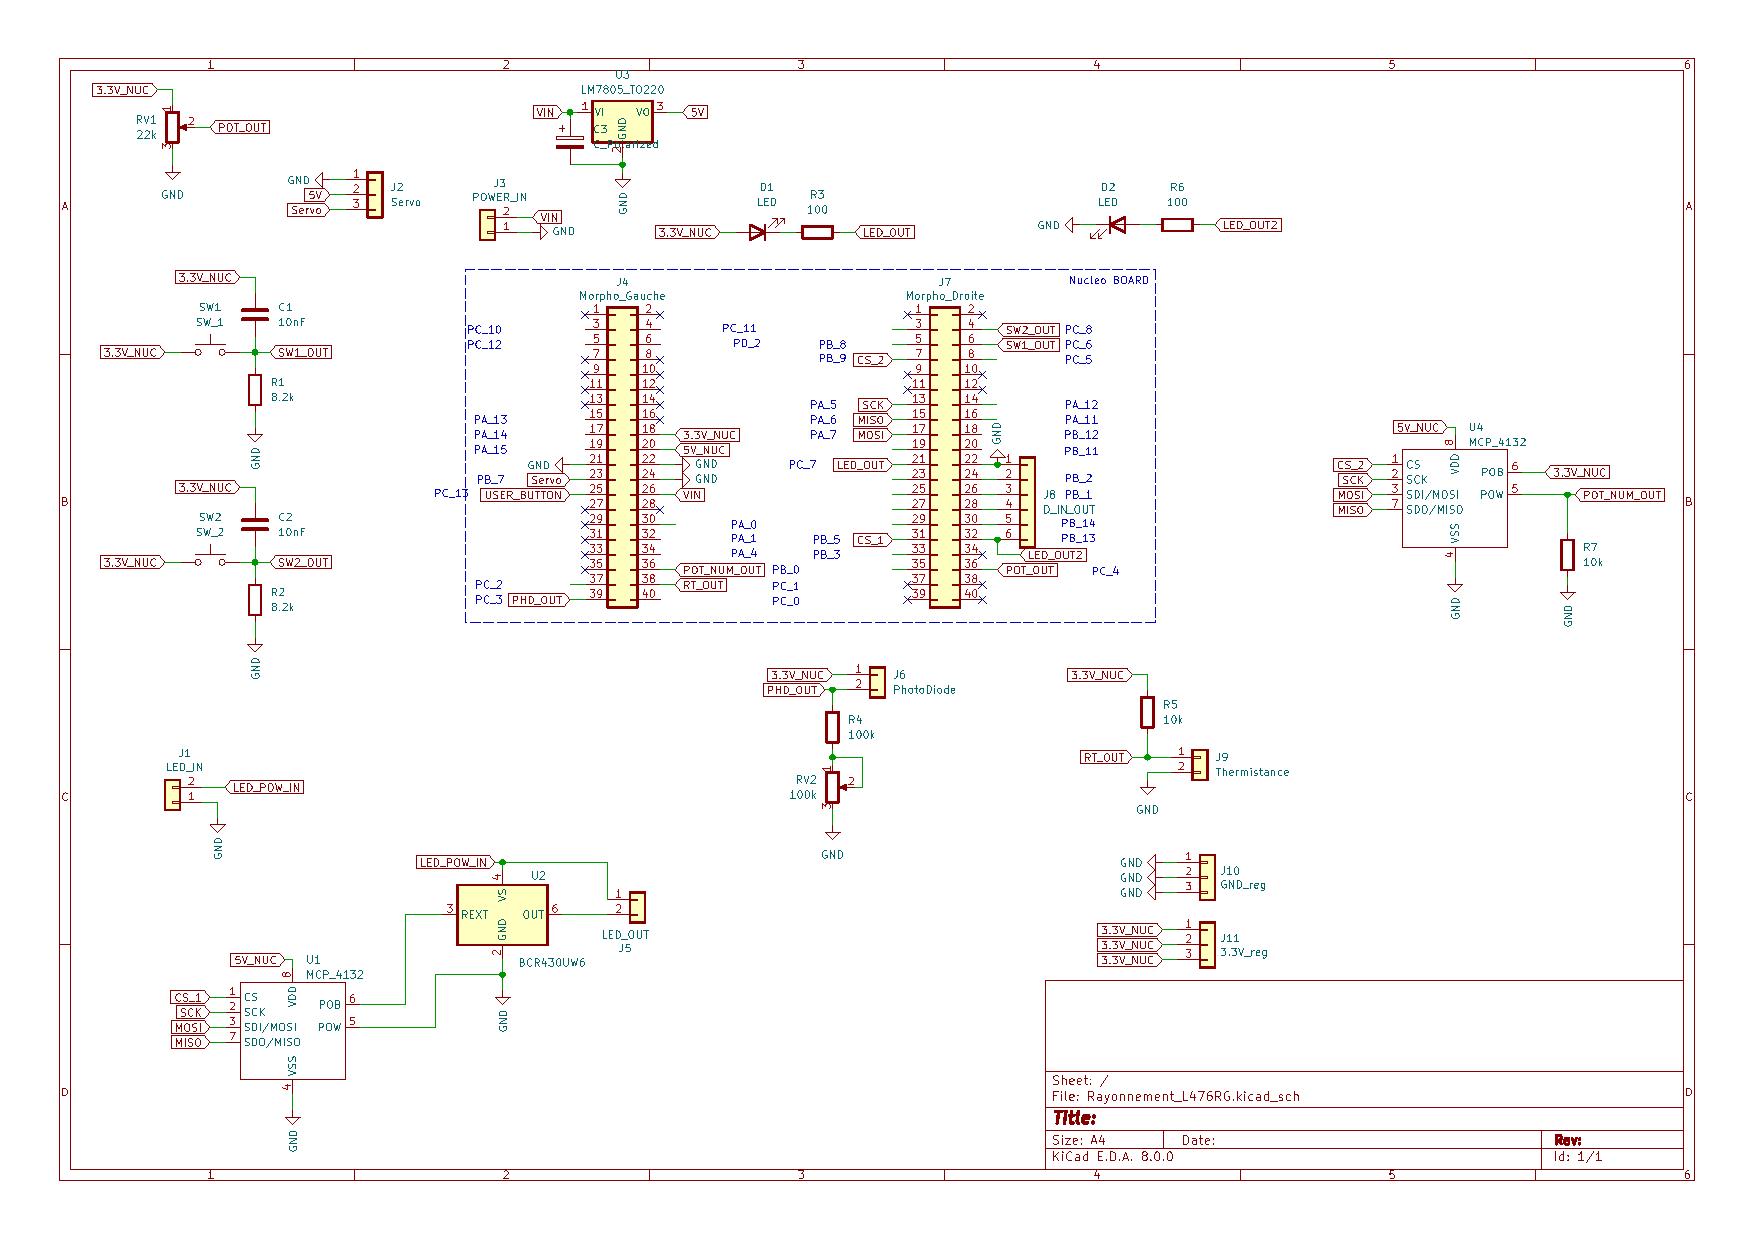
\includepdf[pages=1, landscape=true, pagecommand={\section{\texorpdfstring{\hspace{-1em}}{Schéma Carte Rayonnement}}}\label{doc:robot_schematic}]{ressources/Rayonnement_L476RG_sch.pdf}


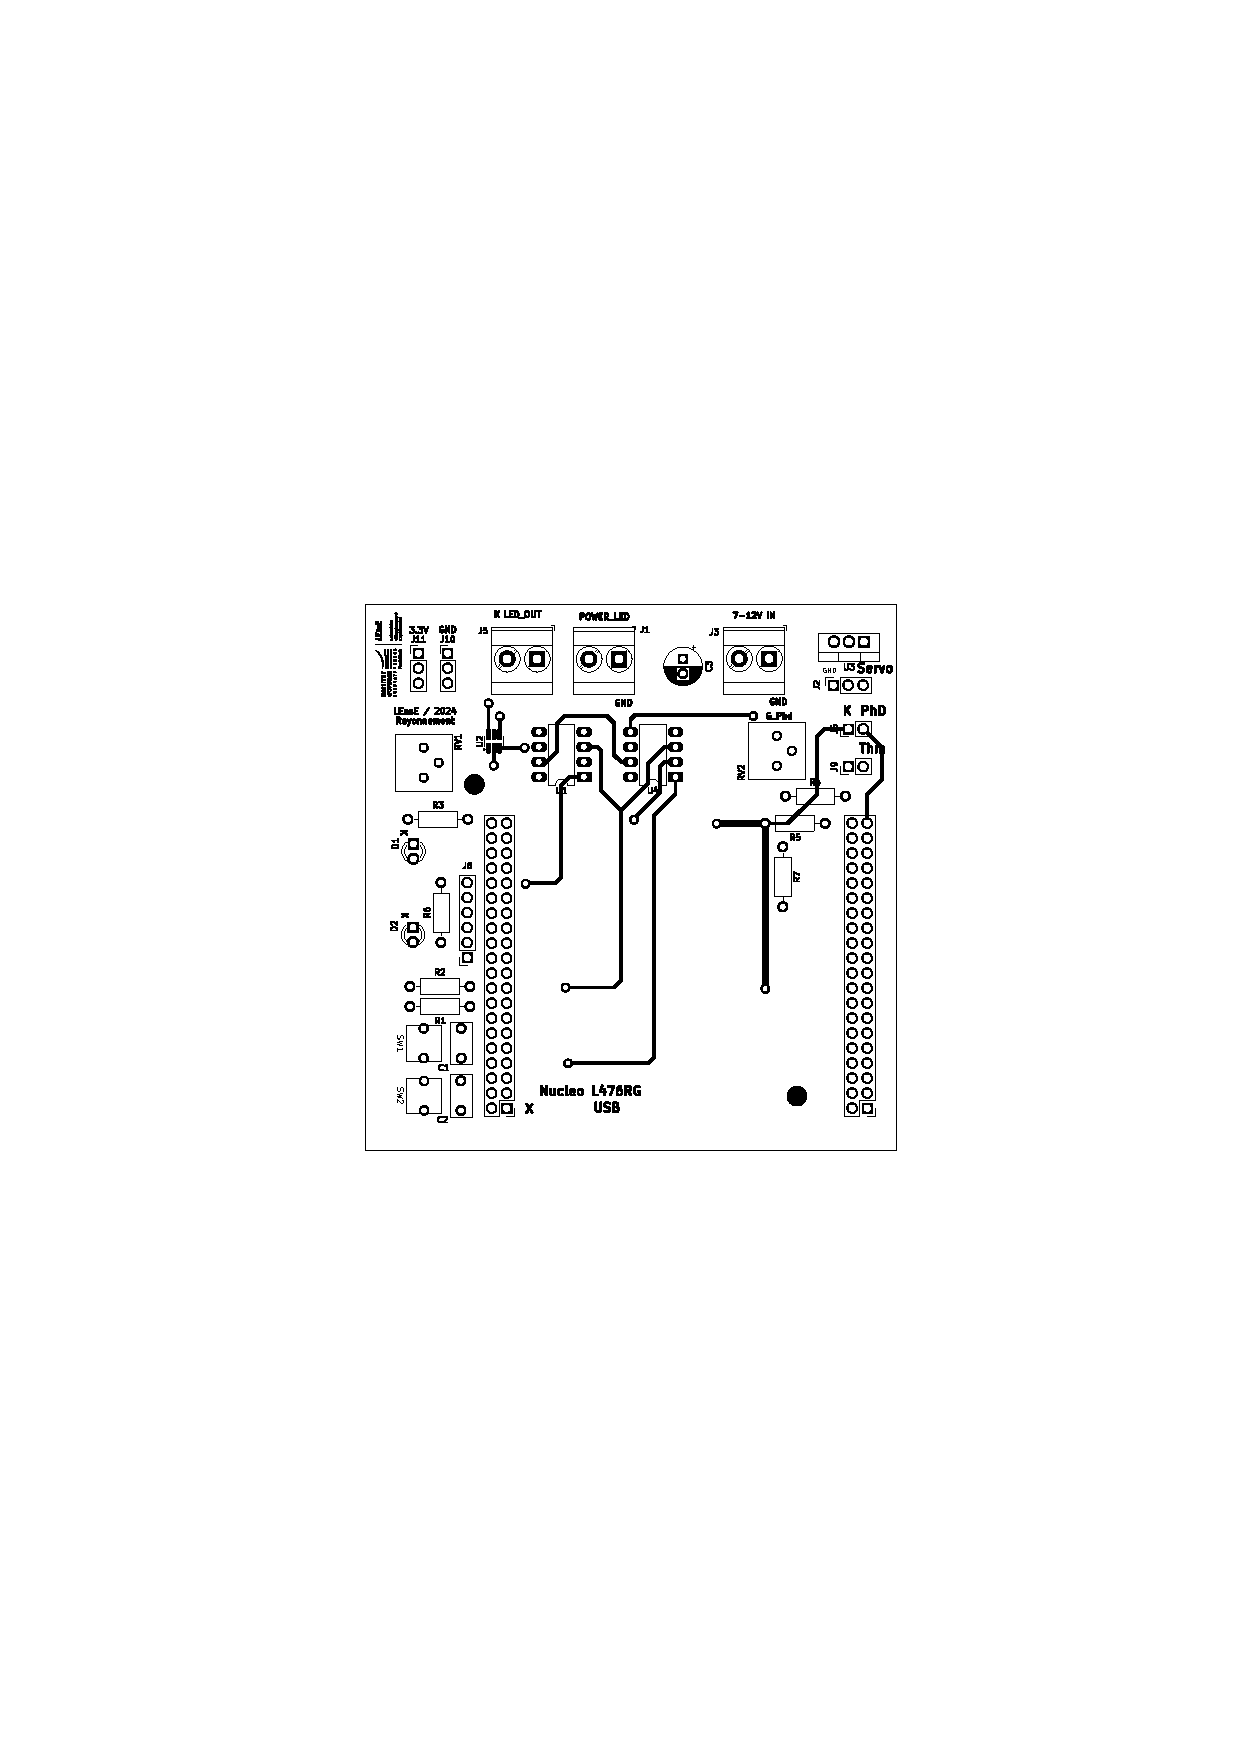
\includepdf[pages=1, pagecommand={\section{\texorpdfstring{\hspace{-1em}}{PCB Carte Rayonnement}}}\label{doc:robot_pcb}]{ressources/Rayonnement_L476RG_pcb.pdf}

\end{document}


